\documentclass{standalone}
\usepackage{tikz}
\usetikzlibrary{patterns, positioning}
\usepackage[sfdefault]{ClearSans} %% option 'sfdefault' activates Clear Sans as the default text font
\usepackage[T1]{fontenc}

\begin{document}
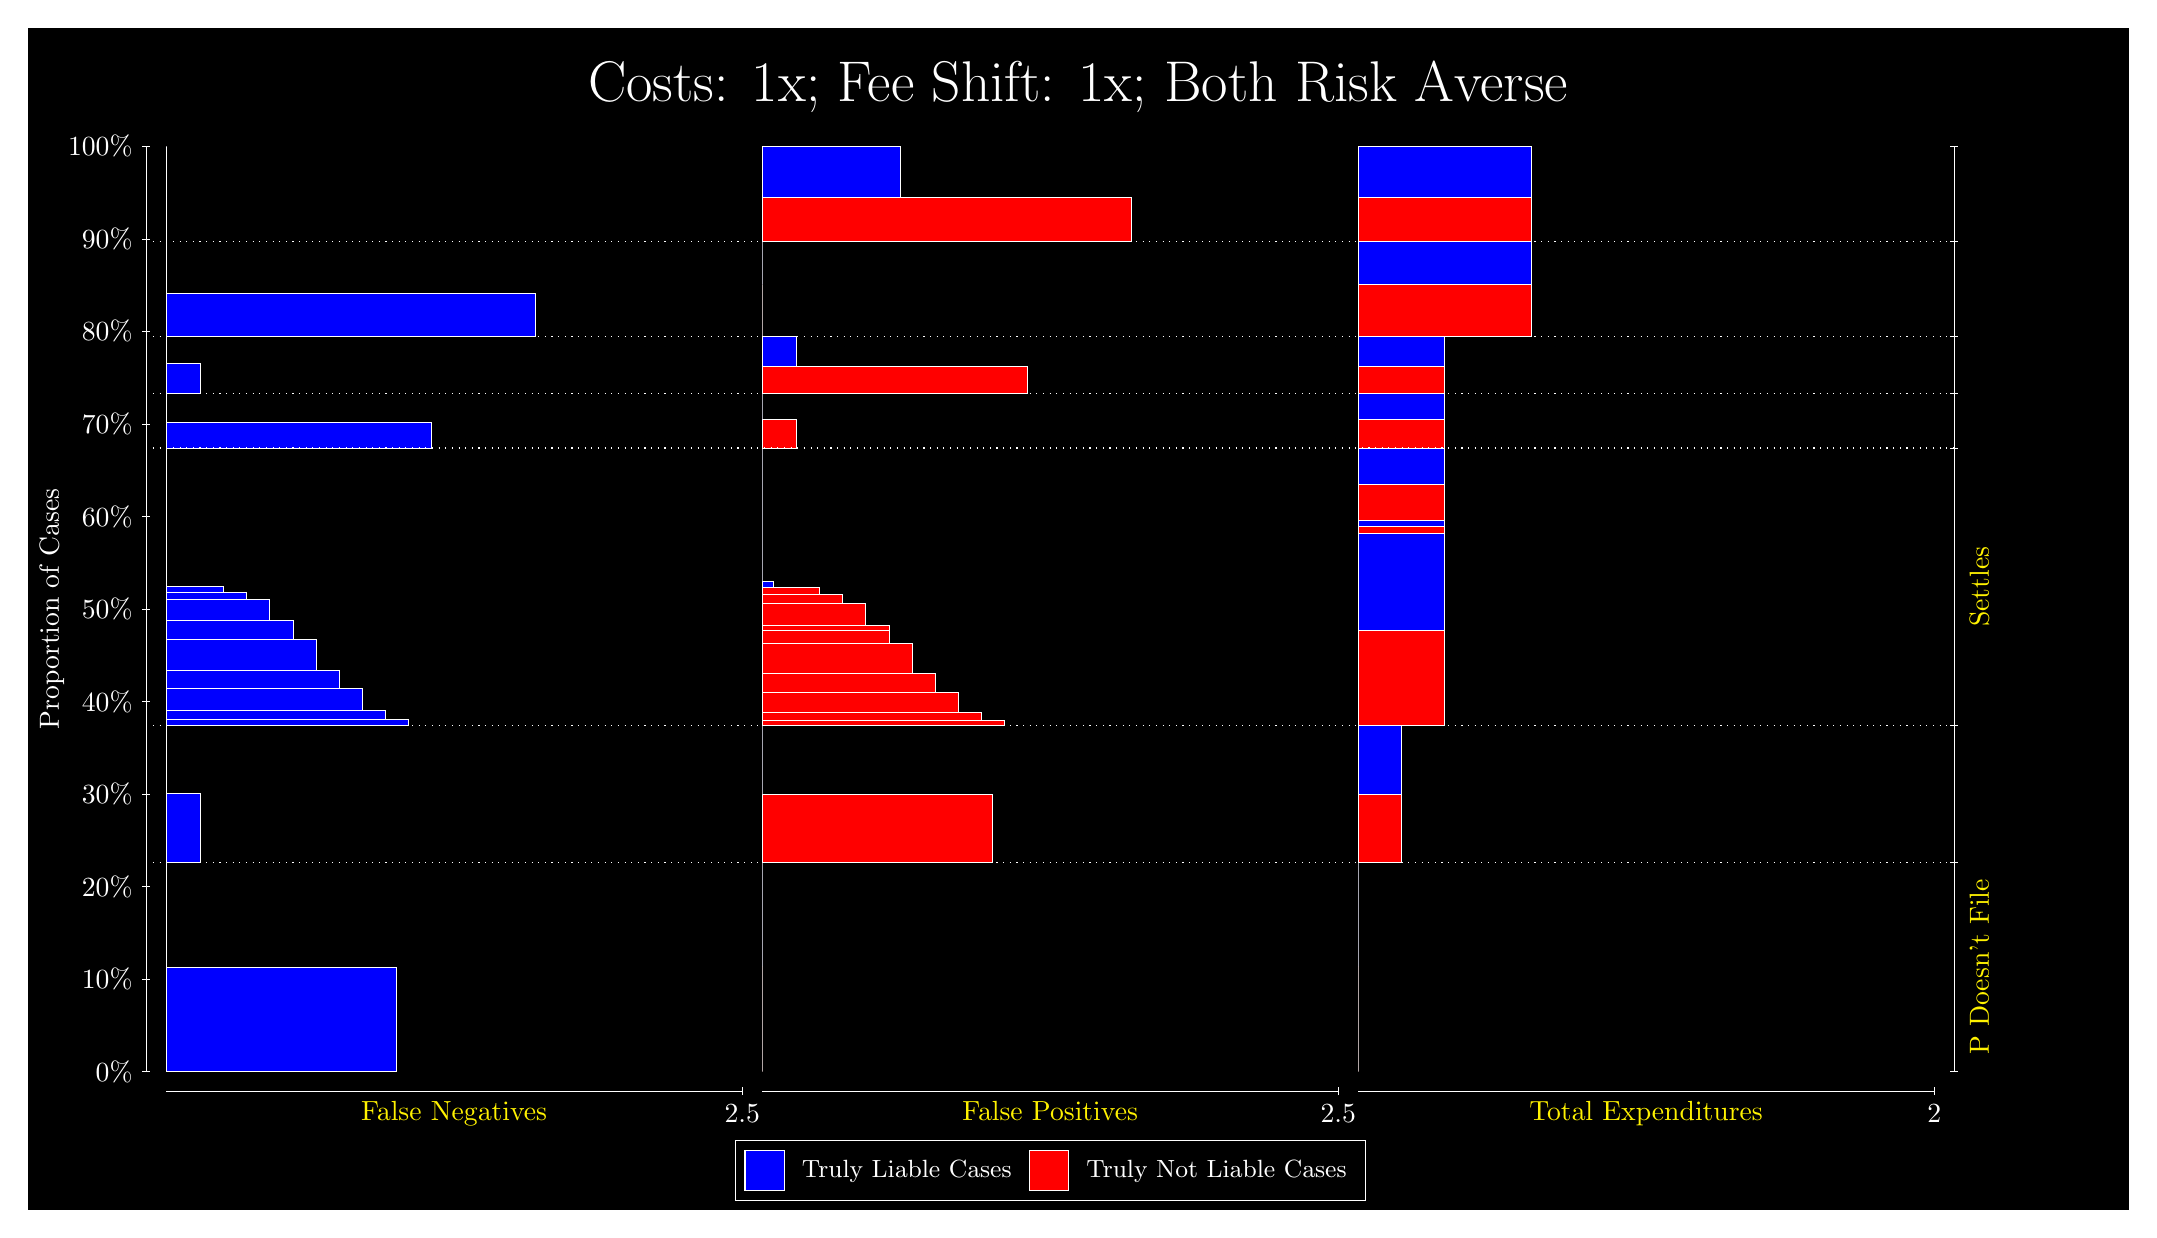
\begin{tikzpicture}
\draw[fill=black] (0,0) rectangle (26.667,15);
\draw[text=white] (0,13.5) rectangle (26.667,15) node[midway] {\huge Costs: 1x; Fee Shift: 1x; Both Risk Averse};
\draw[white, very thin] (1.5,1.75) -- (1.5,13.5);
\node[rotate=90, text=white, anchor=center] at (0.3, 7.625) {Proportion of Cases};
\draw[white, very thin] (1.45,1.75) -- (1.55,1.75);
\node[text=white, anchor=east] at (1.45, 1.75) {0\%};
\draw[white, very thin] (1.45,2.925) -- (1.55,2.925);
\node[text=white, anchor=east] at (1.45, 2.925) {10\%};
\draw[white, very thin] (1.45,4.1) -- (1.55,4.1);
\node[text=white, anchor=east] at (1.45, 4.1) {20\%};
\draw[white, very thin] (1.45,5.275) -- (1.55,5.275);
\node[text=white, anchor=east] at (1.45, 5.275) {30\%};
\draw[white, very thin] (1.45,6.45) -- (1.55,6.45);
\node[text=white, anchor=east] at (1.45, 6.45) {40\%};
\draw[white, very thin] (1.45,7.625) -- (1.55,7.625);
\node[text=white, anchor=east] at (1.45, 7.625) {50\%};
\draw[white, very thin] (1.45,8.8) -- (1.55,8.8);
\node[text=white, anchor=east] at (1.45, 8.8) {60\%};
\draw[white, very thin] (1.45,9.975) -- (1.55,9.975);
\node[text=white, anchor=east] at (1.45, 9.975) {70\%};
\draw[white, very thin] (1.45,11.15) -- (1.55,11.15);
\node[text=white, anchor=east] at (1.45, 11.15) {80\%};
\draw[white, very thin] (1.45,12.325) -- (1.55,12.325);
\node[text=white, anchor=east] at (1.45, 12.325) {90\%};
\draw[white, very thin] (1.45,13.5) -- (1.55,13.5);
\node[text=white, anchor=east] at (1.45, 13.5) {100\%};

\draw[white, very thin] (24.457,1.75) -- (24.457,13.5);
\draw[white, very thin] (24.407,1.75) -- (24.507,1.75);
\node[anchor=west] at (24.407, 1.75) {};
\draw[white, very thin] (24.407,4.4066) -- (24.507,4.4066);
\node[anchor=west] at (24.407, 4.4066) {};
\draw[white, very thin] (24.407,6.1454) -- (24.507,6.1454);
\node[anchor=west] at (24.407, 6.1454) {};
\draw[white, very thin] (24.407,9.669) -- (24.507,9.669);
\node[anchor=west] at (24.407, 9.669) {};
\draw[white, very thin] (24.407,10.358) -- (24.507,10.358);
\node[anchor=west] at (24.407, 10.358) {};
\draw[white, very thin] (24.407,11.088) -- (24.507,11.088);
\node[anchor=west] at (24.407, 11.088) {};
\draw[white, very thin] (24.407,12.296) -- (24.507,12.296);
\node[anchor=west] at (24.407, 12.296) {};
\draw[white, very thin] (24.407,13.5) -- (24.507,13.5);
\node[anchor=west] at (24.407, 13.5) {};

\draw[white, very thin, fill=blue] (1.75,1.75) rectangle (4.6775,3.0687);
\draw[white, very thin, fill=red] (1.75,3.0687) rectangle (1.75,4.4066);
\draw[white, very thin, fill=blue] (1.75,4.4066) rectangle (2.1891,5.2859);
\draw[white, very thin, fill=red] (1.75,5.2859) rectangle (1.75,6.1454);
\draw[white, very thin, fill=blue] (1.75,6.1454) rectangle (4.8239,6.2288);
\draw[white, very thin, fill=blue] (1.75,6.2288) rectangle (4.5312,6.3346);
\draw[white, very thin, fill=blue] (1.75,6.3346) rectangle (4.2384,6.6134);
\draw[white, very thin, fill=blue] (1.75,6.6134) rectangle (3.9457,6.8485);
\draw[white, very thin, fill=blue] (1.75,6.8485) rectangle (3.6529,7.2371);
\draw[white, very thin, fill=blue] (1.75,7.2371) rectangle (3.3602,7.4757);
\draw[white, very thin, fill=blue] (1.75,7.4757) rectangle (3.0674,7.7433);
\draw[white, very thin, fill=blue] (1.75,7.7433) rectangle (2.7746,7.8418);
\draw[white, very thin, fill=blue] (1.75,7.8418) rectangle (2.4819,7.9135);
\draw[white, very thin, fill=red] (1.75,7.9135) rectangle (1.75,9.669);
\draw[white, very thin, fill=blue] (1.75,9.669) rectangle (5.1167,9.9974);
\draw[white, very thin, fill=red] (1.75,9.9974) rectangle (1.75,10.358);
\draw[white, very thin, fill=blue] (1.75,10.358) rectangle (2.1891,10.745);
\draw[white, very thin, fill=red] (1.75,10.745) rectangle (1.75,11.088);
\draw[white, very thin, fill=blue] (1.75,11.088) rectangle (6.4341,11.636);
\draw[white, very thin, fill=red] (1.75,11.636) rectangle (1.75,12.296);
\draw[white, very thin, fill=red] (1.75,12.296) rectangle (1.75,12.855);
\draw[white, very thin, fill=blue] (1.75,12.855) rectangle (1.75,13.5);
\draw[white, very thin, fill=red] (9.3189,1.75) rectangle (9.3189,3.0878);
\draw[white, very thin, fill=blue] (9.3189,3.0878) rectangle (9.3189,4.4066);
\draw[white, very thin, fill=red] (9.3189,4.4066) rectangle (12.246,5.2661);
\draw[white, very thin, fill=blue] (9.3189,5.2661) rectangle (9.3189,6.1454);
\draw[white, very thin, fill=red] (9.3189,6.1454) rectangle (12.393,6.2122);
\draw[white, very thin, fill=red] (9.3189,6.2122) rectangle (12.1,6.3073);
\draw[white, very thin, fill=red] (9.3189,6.3073) rectangle (11.807,6.5703);
\draw[white, very thin, fill=red] (9.3189,6.5703) rectangle (11.515,6.8032);
\draw[white, very thin, fill=red] (9.3189,6.8032) rectangle (11.222,7.1881);
\draw[white, very thin, fill=red] (9.3189,7.1881) rectangle (10.929,7.351);
\draw[white, very thin, fill=red] (9.3189,7.351) rectangle (10.929,7.4229);
\draw[white, very thin, fill=red] (9.3189,7.4229) rectangle (10.636,7.7024);
\draw[white, very thin, fill=red] (9.3189,7.7024) rectangle (10.344,7.8112);
\draw[white, very thin, fill=red] (9.3189,7.8112) rectangle (10.051,7.901);
\draw[white, very thin, fill=blue] (9.3189,7.901) rectangle (9.4652,7.9726);
\draw[white, very thin, fill=blue] (9.3189,7.9726) rectangle (9.3189,9.669);
\draw[white, very thin, fill=red] (9.3189,9.669) rectangle (9.758,10.03);
\draw[white, very thin, fill=blue] (9.3189,10.03) rectangle (9.3189,10.358);
\draw[white, very thin, fill=red] (9.3189,10.358) rectangle (12.686,10.701);
\draw[white, very thin, fill=blue] (9.3189,10.701) rectangle (9.758,11.088);
\draw[white, very thin, fill=red] (9.3189,11.088) rectangle (9.3189,11.747);
\draw[white, very thin, fill=blue] (9.3189,11.747) rectangle (9.3189,12.296);
\draw[white, very thin, fill=red] (9.3189,12.296) rectangle (14.003,12.855);
\draw[white, very thin, fill=blue] (9.3189,12.855) rectangle (11.075,13.5);
\draw[white, very thin, fill=red] (16.888,1.75) rectangle (16.888,3.0878);
\draw[white, very thin, fill=blue] (16.888,3.0878) rectangle (16.888,4.4066);
\draw[white, very thin, fill=red] (16.888,4.4066) rectangle (17.437,5.2661);
\draw[white, very thin, fill=blue] (16.888,5.2661) rectangle (17.437,6.1454);
\draw[white, very thin, fill=red] (16.888,6.1454) rectangle (17.986,7.351);
\draw[white, very thin, fill=blue] (16.888,7.351) rectangle (17.986,8.5807);
\draw[white, very thin, fill=red] (16.888,8.5807) rectangle (17.986,8.6704);
\draw[white, very thin, fill=blue] (16.888,8.6704) rectangle (17.986,8.7538);
\draw[white, very thin, fill=red] (16.888,8.7538) rectangle (17.986,9.2141);
\draw[white, very thin, fill=blue] (16.888,9.2141) rectangle (17.986,9.669);
\draw[white, very thin, fill=red] (16.888,9.669) rectangle (17.986,10.03);
\draw[white, very thin, fill=blue] (16.888,10.03) rectangle (17.986,10.358);
\draw[white, very thin, fill=red] (16.888,10.358) rectangle (17.986,10.701);
\draw[white, very thin, fill=blue] (16.888,10.701) rectangle (17.986,11.088);
\draw[white, very thin, fill=red] (16.888,11.088) rectangle (19.083,11.747);
\draw[white, very thin, fill=blue] (16.888,11.747) rectangle (19.083,12.296);
\draw[white, very thin, fill=red] (16.888,12.296) rectangle (19.083,12.855);
\draw[white, very thin, fill=blue] (16.888,12.855) rectangle (19.083,13.5);
\draw[white, dotted] (1.5,4.4066) -- (24.457,4.4066);
\draw[white, dotted] (1.5,6.1454) -- (24.457,6.1454);
\draw[white, dotted] (1.5,9.669) -- (24.457,9.669);
\draw[white, dotted] (1.5,10.358) -- (24.457,10.358);
\draw[white, dotted] (1.5,11.088) -- (24.457,11.088);
\draw[white, dotted] (1.5,12.296) -- (24.457,12.296);
\draw[white, very thin] (1.75,1.5) -- (9.0689,1.5);
\node[text=yellow, anchor=north] at (5.4094, 1.5) {False Negatives};
\draw[white, very thin] (9.0689,1.45) -- (9.0689,1.55);
\node[text=white, anchor=north] at (9.0689, 1.45) {2.5};

\draw[white, very thin] (9.3189,1.5) -- (16.638,1.5);
\node[text=yellow, anchor=north] at (12.978, 1.5) {False Positives};
\draw[white, very thin] (16.638,1.45) -- (16.638,1.55);
\node[text=white, anchor=north] at (16.638, 1.45) {2.5};

\draw[white, very thin] (16.888,1.5) -- (24.207,1.5);
\node[text=yellow, anchor=north] at (20.547, 1.5) {Total Expenditures};
\draw[white, very thin] (24.207,1.45) -- (24.207,1.55);
\node[text=white, anchor=north] at (24.207, 1.45) {2};

\node[text=yellow, centered, rotate=90] at (24.777, 3.0783) {P Doesn't File};

\node[text=yellow, centered, rotate=90] at (24.777, 7.9072) {Settles};





\draw (12.978300999999998,1.5) node[draw=none] (baseCoordinate) {};
\begin{scope}[align=center]
        \matrix[scale=0.5, draw=white, below=0.5cm of baseCoordinate, nodes={draw}, column sep=0.1cm]{
            \node[rectangle, draw, minimum width=0.5cm, minimum height=0.5cm, fill=blue] {}; &
            \node[draw=none, font=\small, text=white] (B) {Truly Liable Cases}; &
            \node[rectangle, draw, minimum width=0.5cm, minimum height=0.5cm, fill=red] {}; &
            \node[draw=none, font=\small, text=white] (B) {Truly Not Liable Cases}; \\
            };
\end{scope}

\end{tikzpicture}
\end{document}